\documentclass[sigconf,anonymous]{acmart}
\usepackage{amsmath}
\usepackage{booktabs}
\usepackage{tabularx}
\usepackage{balance}
\usepackage{siunitx}
\sisetup{group-minimum-digits=4,group-separator={,}}
\settopmatter{printacmref=false,printfolios=true,printccs=false}
\setlength{\emergencystretch}{1.5em}
\vfuzz=2pt
\setcopyright{none}
\renewcommand\footnotetextcopyrightpermission[1]{}
\acmConference[SIGMOD 2027]{SIGMOD 2027}{Under review}{Anonymous submission}
\acmBooktitle{SIGMOD 2027 Experiments \& Analysis submission}
\acmYear{2027}
\copyrightyear{2027}
\acmDOI{}
\acmISBN{}
\newcommand{\risk}{\mathcal{R}}
\newcommand{\ndc}{\operatorname{NDC}}
\newcommand{\rec}{\operatorname{Recall}}
\newcommand{\indicator}{\mathbf{1}}
\newcommand{\slot}[2]{%
  \fbox{\parbox{\dimexpr\linewidth-2\fboxsep-2\fboxrule\relax}{%
  \small\textbf{Planned exhibit: #1}\par\medskip #2}}}
\newcommand{\sectionaim}[1]{\noindent\textit{Section purpose: #1}\par}

\newcommand{\GraphOnlyRows}{%
hnswlib HNSW & SIFT & 22.31 & 0.77 & 21.55 [20.76, 22.33] & 89.33 \\
Faiss HNSW & SIFT & 23.67 & 0.07 & 23.60 [22.78, 24.39] & 91.07 \\
hnswlib HNSW & Arxiv & 18.24 & 1.07 & 17.17 [16.33, 18.06] & 75.87 \\
Faiss HNSW & Arxiv & 17.93 & 0.17 & 17.77 [16.86, 18.68] & 75.87 \\
}
\newcommand{\RecoveryRows}{%
SIFT & Endpoint & 0.97 [0.53, 1.50] & 0.00 [0.00, 0.00] & 1,826 & 2,615 & 2,855 \\
SIFT & Direct reuse & 6.69 [5.65, 7.77] & 59.51 [57.83, 61.20] & 739 & 2,132 & 2,706 \\
SIFT & Original recalibration & 1.79 [1.25, 2.40] & 44.39 [42.76, 46.01] & 1,015 & 2,349 & 2,774 \\
SIFT & Joint-error replay & 1.79 [1.25, 2.40] & 44.39 [42.76, 46.01] & 1,015 & 2,349 & 2,774 \\
\addlinespace
Arxiv & Endpoint & 1.01 [0.61, 1.47] & 0.00 [0.00, 0.00] & 2,397 & 3,252 & 3,504 \\
Arxiv & Direct reuse & 7.24 [6.18, 8.36] & 64.21 [62.51, 65.85] & 858 & 2,586 & 3,322 \\
Arxiv & Original recalibration & 2.04 [1.45, 2.69] & 44.79 [34.32, 50.96] & 1,323 & 2,974 & 3,398 \\
Arxiv & Joint-error replay & 1.68 [1.10, 2.35] & 29.86 [14.75, 45.00] & 1,681 & 3,117 & 3,460 \\
\addlinespace
}
\newcommand{\CostRows}{%
SIFT & Cached & 129 [129, 129] & 0/10 \\
SIFT & Cold & 396 [395, 397] & 0/10 \\
Arxiv & Cached & 148 [99, 296] & 4/10 \\
Arxiv & Cold & 457 [305, 915] & 4/10 \\
}
\newcommand{\CertificateRows}{%
S & 1103 & 1 & 9 & 3.12 & 3.39 & 2 & 1.44 & C & 1.50 & 44.33 \\
S & 1229 & 1 & 8 & 2.87 & 3.13 & 5 & 2.32 & C & 1.90 & 44.28 \\
S & 1361 & 1 & 10 & 3.37 & 3.65 & 2 & 1.44 & C & 1.80 & 44.29 \\
S & 1499 & 1 & 6 & 2.35 & 2.59 & 3 & 1.74 & C & 2.00 & 44.51 \\
S & 1621 & 1 & 8 & 2.87 & 3.13 & 5 & 2.32 & C & 1.90 & 44.39 \\
S & 1747 & 1 & 11 & 3.62 & 3.90 & 2 & 1.44 & C & 1.90 & 44.28 \\
S & 1877 & 1 & 8 & 2.87 & 3.13 & 4 & 2.04 & C & 1.80 & 44.36 \\
S & 1999 & 1 & 8 & 2.87 & 3.13 & 4 & 2.04 & C & 1.70 & 44.35 \\
S & 2131 & 1 & 6 & 2.35 & 2.59 & 2 & 1.44 & C & 1.70 & 44.53 \\
S & 2267 & 1 & 10 & 3.37 & 3.65 & 2 & 1.44 & C & 1.70 & 44.61 \\
A & 1103 & 1 & 14 & 4.34 & 4.65 & 6 & 2.59 & C & 2.20 & 49.77 \\
A & 1229 & 1 & 17 & 5.06 & 5.39 & 5 & 2.32 & E & 1.30 & 0.00 \\
A & 1361 & 1 & 14 & 4.34 & 4.65 & 3 & 1.74 & C & 2.30 & 49.76 \\
A & 1499 & 1 & 16 & 4.82 & 5.14 & 4 & 2.04 & E & 0.90 & 0.00 \\
A & 1621 & 1 & 16 & 4.82 & 5.14 & 6 & 2.59 & E & 1.10 & 0.00 \\
A & 1747 & 1 & 15 & 4.58 & 4.90 & 6 & 2.59 & C & 1.50 & 49.84 \\
A & 1877 & 1 & 13 & 4.10 & 4.41 & 1 & 1.11 & C & 1.80 & 49.68 \\
A & 1999 & 1 & 13 & 4.10 & 4.41 & 5 & 2.32 & C & 2.20 & 49.80 \\
A & 2131 & 1 & 15 & 4.58 & 4.90 & 5 & 2.32 & C & 2.50 & 49.87 \\
A & 2267 & 1 & 16 & 4.82 & 5.14 & 5 & 2.32 & E & 1.00 & 0.00 \\
}
\newcommand{\SensitivityRows}{%
SIFT & Original & [42.76, 46.01] & [44.33, 44.47] & [42.86, 46.07] \\
SIFT & Joint & [42.76, 46.01] & [44.33, 44.47] & [42.86, 46.07] \\
Arxiv & Original & [34.32, 50.96] & [34.82, 49.81] & [43.27, 46.27] \\
Arxiv & Joint & [14.75, 45.00] & [14.92, 44.80] & [28.85, 30.84] \\
}

% Generated by evidence/check_postseal.py from packaged post-seal evidence.
\newcommand{\TargetCertifiedRows}{%
SIFT & 552/0/0 & 0.126 [0.040, 0.250] & 8.283 [7.921, 8.557] & 0.9964 / 0.9987 & 8.267 \\
Arxiv & 552/0/0 & 0.530 [0.233, 0.915] & 29.083 [28.653, 29.518] & 0.9797 / 0.9828 & 29.027 \\
}
\newcommand{\TargetStageCostRows}{%
SIFT & Pairwise & 552 & 66,914 [64,805, 69,940] & 460 & 100,000 \\
SIFT & Shared target & 24 & 3,019 [2,923, 3,157] & 0 & 10,000 \\
Arxiv & Pairwise & 552 & 17,018 [16,767, 17,276] & 230 & 100,000 \\
Arxiv & Shared target & 24 & 755 [744, 767] & 0 & 1,000 \\
}

\newcommand{\SProspectiveRows}{%
SIFT & 56/0/0 & 0.475 [0.125, 0.950] & 51.35 [50.87, 51.84] & 0.519 [0.509, 0.528] & 51.19 \\
Arxiv & 56/0/0 & 0.536 [0.146, 1.068] & 30.13 [28.64, 31.88] & 0.891 [0.855, 0.917] & 29.49 \\
}
\newcommand{\SStrongBaselineRows}{%
SIFT & Fixed-256 & 56/0/0 & 0.400 [0.050, 0.925] & 51.93 [51.20, 52.79] & 0.515 [0.505, 0.525] & 51.61 \\
SIFT & Source one-rung & 56/0/0 & 0.400 [0.050, 0.925] & 51.93 [51.20, 52.79] & 0.515 [0.505, 0.525] & 51.61 \\
SIFT & Target-global-500 & 49/7/0 & 0.350 [0.025, 0.850] & 45.33 [32.48, 52.00] & 0.834 [0.509, 0.930] & 44.26 \\
SIFT & Target-global-1000 & 56/0/0 & 0.725 [0.100, 1.625] & 54.53 [51.20, 60.56] & 0.513 [0.502, 0.524] & 51.61 \\
Arxiv & Fixed-256 & 56/0/0 & 0.400 [0.100, 0.750] & 43.64 [43.33, 43.97] & 0.563 [0.557, 0.574] & 43.57 \\
Arxiv & Source one-rung & 56/0/0 & 0.307 [0.089, 0.575] & 32.73 [31.09, 34.55] & 0.868 [0.843, 0.891] & 32.05 \\
Arxiv & Target-global-500 & 49/7/0 & 0.925 [0.300, 1.800] & 46.81 [30.36, 60.54] & 0.763 [0.500, 0.921] & 43.96 \\
Arxiv & Target-global-1000 & 56/0/0 & 2.225 [1.325, 3.300] & 66.47 [66.20, 66.74] & 0.340 [0.334, 0.346] & 66.43 \\
}

\hypersetup{pdfauthor={},pdfsubject={Graph-ANNS budget portability, risk auditing, and target recalibration},pdfkeywords={graph ANNS, budget transfer, risk auditing, target recalibration}}

\title[Auditing Search-Budget Portability]{Auditing Search-Budget Portability Across Graph-ANNS Rebuilds: [Experiments \& Analysis]}
\author{Anonymous Author(s)}
\begin{document}
\begin{abstract}
Graph indexes are rebuilt while their search-budget policies are often retained. On the registered SIFT-100K and Arxiv-Nomic-100K build panels, action grids, and query populations, transferred first-passing actions add 17.17--23.60 percentage points of query failure above target-specific references; after a 5\% data refresh, a fixed recurring-query policy crosses a 5\% risk limit. Index-Conditioned Budget Audit (ICBA) turns reuse into a target decision by separating policy construction, certification, fallback, held-out evaluation, and acquisition cost. Target-calibrated pooling (TCP) reduces endpoint-relative distance work by 44.39\% and 29.86\%, although its incremental advantage over target calibration with the same target-label budget is resolved only on SIFT. On a prospective insertion-permutation panel, the frozen candidate separately qualifies in all 112 fixed target decisions under per-decision certificates and reduces measured wall-time by 51.35\% and 30.13\% on one fixed CPU setting; this is not a simultaneous campaign certificate. A paired audit then shows that a certified fixed action matches the source one-rung candidate on SIFT and is more efficient on Arxiv under the same risk contract, while label-richer target calibration gives the largest measured reductions. ICBA is therefore the central contribution: deploy the least complex target-qualified policy whose information cost is justified by held-out value.
\end{abstract}
\keywords{approximate nearest-neighbor search, graph indexes, index rebuilding, risk auditing, budget transfer}
\maketitle
\raggedbottom

\section{Introduction}
\label{sec:intro}

A graph index and its search-budget policy jointly determine approximate nearest-neighbor search (ANNS) quality and cost. Rebuilding an HNSW or Vamana index changes traversal paths even when vectors and queries are unchanged; refreshing data also changes nearest-neighbor truth~\cite{malkov2020hnsw,subramanya2019diskann}. A retained budget is therefore versioned decision state, not inert configuration.

The relevant failure is query-level: $\rec@10<0.95$. Because recall is discrete, one missed neighbor is a failure. A 5\% risk limit asks that at least 95\% of queries return all ten neighbors. This differs from mean recall and exposes two effects that averages can hide: target queries unresolved even at the endpoint, and additional failure caused by a transferred action.

We ask: \emph{what target evidence is required before a budget policy can be reused?} On the registered builds, grids, and query populations, graph-only transfer on unchanged collections adds 17.17--23.60 percentage points of failure above target-specific references across hnswlib and Faiss. After a 5\% data refresh, a fixed recurring-query policy crosses the declared 5\% risk limit on both datasets. Prospective experiments then test which recovery policies are qualified, lower-latency, and stable on the registered build panels.

\emph{Index-Conditioned Budget Audit} (ICBA) is the resulting decision contract. It declares the target index, workload, native action grid, failure event, permitted observations, candidate policy, target certificate, fallback, held-out evaluation, and acquisition ledger. This separation prevents four different claims---portability, qualification, serving gain, and lifecycle value---from being collapsed into one number.

We evaluate a hierarchy of recovery policies. A fixed action is the minimum-complexity baseline. Target-global calibration chooses one action using target labels. \emph{Target-calibrated pooling} (TCP) uses recurring-query histories and one target-selected global shift to retain query conditioning. In the incremental comparison, TCP and target-global receive the same target-label budget, while TCP additionally uses nine historical per-query profiles. A \emph{source one-rung} rule shifts a source-qualified action upward by one native grid level; it is a diagnostic bridge, not a presumed improvement over simpler policies.

The resulting evidence supports a policy ladder rather than one universal recovery algorithm. TCP has endpoint-relative value on both datasets, but its incremental value over target calibration with the same target-label budget is resolved only on SIFT. On a prospective panel, source one-rung qualifies and lowers latency; a paired audit on the same builds then shows that fixed-256 matches it on SIFT and provides greater efficiency on Arxiv while both satisfy the risk contract. Label-richer target calibration achieves the largest measured reduction. The operational rule is to deploy the least complex target-qualified policy that meets the target service-level agreement (SLA).

\begin{figure*}[t]
\centering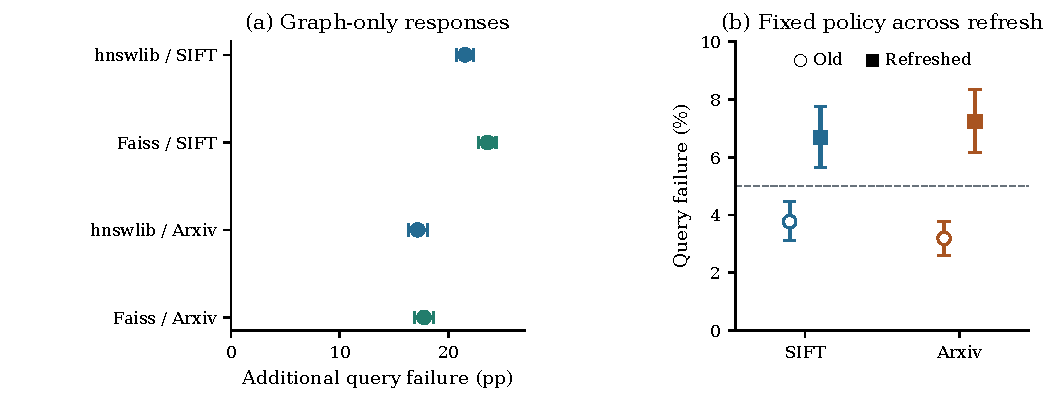
\includegraphics[width=\textwidth]{figures_v3/overview.pdf}
\caption{Two failures that motivate ICBA. Left: graph-only transfer of retrospective first-passing actions, with a query-cluster interval conditional on fixed builds. Right: one executable recurring-query policy before and after a 5\% refresh, with a crossed target-build/query interval.}
\label{fig:overview}
\Description{Four graph-only incremental-risk estimates are positive. In the refresh test, risk increases on both datasets and crosses five percent.}
\end{figure*}

\begin{table}[t]
\caption*{\textbf{Terms at a glance.} Tables shorten Arxiv-Nomic-100K to Arxiv.}
\small\begin{tabularx}{\linewidth}{@{}lX@{}}\toprule
Term & Meaning \\\midrule
ICBA & Audit contract for target portability and deployment.\\
TCP & Target-calibrated pooling for recurring profiled queries.\\
Action & One native search-budget value.\\
Policy & Rule mapping permitted observations to an action.\\
Candidate & Frozen policy/action awaiting certification.\\
Target-qualified & Candidate whose target certificate passes.\\
Target-certified stage & Protocol stage that checks frozen target candidates.\\
Accepted & Completed decision executes the qualified candidate.\\
Completed decision & Executed candidate, fallback, or abstention.\\
NDC & Number of distance calculations.\\
CP / UCB & Clopper--Pearson / upper confidence bound.\\
LOTO & Leave one target build out.\\
Endpoint & Largest registered native action.\\\bottomrule
\end{tabularx}
\end{table}

We make three contributions. First, across the registered panels we establish budget non-portability under graph-only rebuilds and data refresh, with scoped extensions across implementations, graph families, and 100K-to-1M scale that retain each setting's estimand. Second, ICBA supplies a reusable protocol that separates response evidence, target qualification, completed execution, and information cost. Third, a preregistered recovery and baseline program identifies when complexity is warranted: target calibration is beneficial on the registered prospective panels, TCP adds resolved query-conditional value on SIFT, and a simple fixed action can match or outperform a source-tailored heuristic under the common risk contract. The artifact regenerates the paper, validates the decision chain, and preserves query-role boundaries.

The systems implication is direct: version the budget policy with its index and workload; qualify reuse on the target; and escalate from fixed to target-global to query-conditional policies only when the measured gain justifies their information cost.

\section{Related Work and Positioning}
\label{sec:related}

\paragraph{Graph construction, evaluation, and maintenance.}
HNSW combines hierarchical navigation with graph search, while DiskANN introduces Vamana as part of a system for large-scale search~\cite{malkov2020hnsw,subramanya2019diskann}. Graph-search evaluations compare construction paradigms across datasets and scales~\cite{azizi2025evaluation}, and insertion order and intrinsic dimensionality affect HNSW recall~\cite{elliott2024ordering}. These studies establish construction sensitivity. We study the decision that survives construction: an action or policy transferred from a source build to a target, with target difficulty separated from additional transfer loss. FreshDiskANN supports streaming updates~\cite{singh2021freshdiskann}; IP-DiskANN performs insertions and deletions in place~\cite{xu2025ipdiskann}; Wolverine repairs monotonic search paths disrupted by deletion~\cite{liu2025wolverine}. These systems change the maintained graph. ICBA evaluates the validity of a budget decision on the graph that maintenance produces.

\paragraph{Adaptive work allocation and declarative recall.}
LAET predicts query-specific termination conditions using static and intermediate-search features~\cite{li2020laet}. DARTH predicts achieved recall during execution and adapts prediction intervals to terminate HNSW or IVF searches at a declarative target~\cite{chatzakis2025darth}. ANNiE estimates the work needed for a recall target from graph-derived features; ANNiE-S uses those estimates directly~\cite{wang2026annie}. Ada-ef models query-to-dataset similarity distributions to choose an HNSW exploration parameter and updates its statistics after insertions or deletions~\cite{zhang2026adaef}. Portability concerns the validity and cost of carrying any such decision between builds. Our frozen DARTH and Ada-ef integrations retain their permitted signals and update procedures, so they test qualification in those settings rather than define a common ranking.

\paragraph{Quality guarantees and their target quantities.}
ConANN applies conformal risk control to IVF search, controlling expected false-negative rate while adapting the number of probed clusters~\cite{horchidan2025conann}. Its objective is the expected fraction of missed neighbors, whereas our principal event is whether a query falls below a recall threshold. ANNiE's optional recall-target guarantee addresses the fraction of queries reaching the requested recall using quantile-loss minimization~\cite{wang2026annie}. The DARTH+ preprint also introduces optional probabilistic quality guarantees for HNSW and IVF~\cite{chatzakis2026darthplus}. We study which build and policy an assessment covers, what information is reused or reacquired, and how the assessed decision behaves after rebuilding. Each comparison therefore retains its original risk quantity.

\paragraph{Calibration, selection, and the role of ICBA.}
Conformal risk control bounds an expected monotone loss under its calibration assumptions~\cite{angelopoulos2024crc}. Learn then Test formulates risk-controlled parameter selection as multiple hypothesis testing~\cite{angelopoulos2021ltt}. These are statistical foundations for auditing a search decision. ConANN explicitly aligns calibration with index construction and assumes exchangeable query data~\cite{horchidan2025conann}; rebuilding can change the loss induced by search even when the query population is retained. ICBA makes the target build, failure event, candidate construction, certification, and fallback rule explicit. TCP and source one-rung instantiate two information patterns within that audit. This separation identifies when target information restores search efficiency and whether the resulting work saving repays its acquisition cost.

\section{Portability, Risk, and the Scope of Guarantees}
\label{sec:theory}

\subsection{Execution Risk and Retrospective Responses}
Let $G$ specify a vector snapshot, graph, and search implementation, and let $\mathcal A=(a_1<\cdots<a_J)$ be its native action grid. A policy $\pi$ maps permitted query and history observations to an action. For $q\sim\mathcal Q$,
\begin{equation}
 \begin{aligned}
 Z_G(q,a)&=\indicator\{\rec@k(G,q,a)<\tau\},\\
 \risk_G(\pi)&=\mathbb E_q Z_G(q,\pi(q)).
 \end{aligned}\label{eq:risk}
\end{equation}
Truth is computed against the corresponding snapshot. We distinguish target transport risk $\risk_{G_t}(\pi_s)$, source risk $\risk_{G_s}(\pi_s)$, and a reference-relative increment
\begin{equation}
 \Delta_{s\to t}=\risk_{G_t}(\pi_s)-\risk_{G_t}(\pi_t^{\rm ref}).\label{eq:increment}
\end{equation}
A matched old-to-new comparison instead subtracts $\risk_{G_s}(\pi_s)$, keeping the policy fixed. These two differences answer different questions.

A retrospective first-passing label is $B_G^{\rm first}(q)=\min\{a_j:Z_G(q,a_j)=0\}$. A stable-tail label is
\begin{equation}
 B_G^{\rm tail}(q)=\min\{a_j:Z_G(q,a_\ell)=0\text{ for every }\ell\ge j\}.\label{eq:stable-label}
\end{equation}
Both require query truth; an empty set is $+\infty$, an unresolved label. Native action order need not make either raw recall or realized NDC monotone. Consequently, an action larger than a first-passing label need not succeed, whereas a finite stable-tail label establishes success above it on the recorded grid. The graph-only study uses first-passing labels and evaluates the transferred action's \emph{actual} target response, rather than replacing execution failure by a budget-order comparison.

\subsection{Information Limits Explain What Must Be Observed}
\label{sec:information-limit}
The following classical two-point argument~\cite{yu1997assouad} states why source information alone may be insufficient. For two environments $E_0,E_1$, let $O$ include everything available to the decision rule, with laws $P_0^O,P_1^O$. Suppose acceptable risk--cost decisions form disjoint sets $D_0,D_1$, and loss satisfies $L_i(a)\ge\lambda\indicator\{a\notin D_i\}$ for $\lambda>0$. Then every common decision rule satisfies
\begin{equation}
 \max_i\mathbb E_i L_i(A)\ge\frac{\lambda}{2}\bigl(1-\operatorname{TV}(P_0^O,P_1^O)\bigr).\label{eq:information}
\end{equation}
Indeed, deciding whether $A\in D_0$ defines a test of the environment; its sum of error probabilities is at least $1-\operatorname{TV}$. If a common expensive endpoint is acceptable, disjointness fails and the bound can be vacuous. For random queries, $O$ must include the query jointly with its transcript. Our measurements establish response differences, not an estimate of full-observation total variation or an impossibility result for every policy. The bound explains the information question; the audit below supplies the operational test. \emph{Takeaway: source observations alone cannot generally identify a low-cost target-qualified action.}

\subsection{Certifying a Fixed-Target Decision}
\label{sec:fixed-cert}
For a policy fixed independently of $n$ i.i.d. target-certification queries, $x$ failures yield the one-sided Clopper--Pearson bound~\cite{clopper1934confidence}
\begin{equation}
 U(x,n;\alpha)=\begin{cases}
 \operatorname{Beta}^{-1}(1-\alpha;x+1,n-x),&x<n,\\1,&x=n.
 \end{cases}\label{eq:cp}
\end{equation}
Acceptance requires $U\le\delta$. Confidence error $\alpha$ and allowed query risk $\delta$ are distinct. At zero failures, $U=1-\alpha^{1/n}$; $\alpha=\delta=0.05$ requires at least 59 queries for acceptance to be possible. With 500 certification queries, nonzero failures can be accepted, but rejection can still reflect limited power near the boundary.

\begin{proposition}[Jointly qualified selection on one target]
\label{prop:simultaneous}
Freeze $K$ policies before certification, and allocate $\alpha_j>0$ with $\sum_{j=1}^K\alpha_j\le\alpha$. On a common i.i.d. certification sample, compute $U_j=U(x_j,n;\alpha_j)$. Select any policy with $U_j\le\delta$, or abstain if none qualifies. Then
\begin{equation}
 \Pr\{\text{a policy is selected and }\risk_G(\pi_{\rm selected})>\delta\}\le\alpha.\label{eq:simultaneous}
\end{equation}
\end{proposition}
\begin{proof}
By a union bound, $\Pr\{\exists j:\risk_G(\pi_j)>U_j\}\le\sum_j\alpha_j$. Otherwise every selectable policy satisfies the risk limit. Independence among policies' bounds is unnecessary.
\end{proof}
This is simultaneous risk control~\cite{angelopoulos2021ltt}. Selection may define the policies using a separate role; the proposition then applies conditionally on selection. A fallback must be included or separately justified. The statement is per fixed target, not simultaneous over a campaign, and does not bound risk conditional on the event of acceptance. Campaign-level coverage would require a separately preregistered simultaneous-error allocation and is not claimed here. The i.i.d. query interpretation concerns the represented workload; fixed-profile replay by itself proves no guarantee for a changed query population. \emph{Takeaway: once candidates are frozen, independent target queries can qualify the completed candidate/fallback decision.}

\subsection{Why Pooling Is Not the Same Certificate}
\label{sec:pooling-theory}
For $m$ source builds and one target with exchangeable budget labels at a fixed query, conformal rank reasoning~\cite{angelopoulos2023conformal} gives a different guarantee. Let $r=\lceil(1-\eta)(m+1)\rceil$. Use the $r$th source order statistic if $r\le m$ and it is finite; otherwise abstain. Then
\begin{equation}
 \Pr\{a(q)<\infty,\ B_t(q)>a(q)\}\le\frac{m+1-r}{m+1}\le\eta.\label{eq:pooling}
\end{equation}
This is build-marginal label coverage for a fixed query. It translates to execution failure for stable-tail labels, but not automatically for first-passing labels. Nine sources offer rank resolution $1/10$, and old/refreshed builds need not be exchangeable. Accordingly, TCP's nine-history replay derives its target qualification from Equation~\eqref{eq:simultaneous}, not from a 5\% conformal claim. The short supplement supplies the rank proof and a margin-based selection result, and states which assumptions are uninstantiated in the experiment. \emph{Takeaway: history pooling constructs a candidate; it does not itself provide the target certificate.}

\section{ICBA and the Recovery Hierarchy}
\label{sec:auditor}

\subsection{The Audit Contract}
ICBA leaves graph construction and native traversal unchanged. Its input declares source and target snapshots, implementation, query population, action grid, permitted observations, failure event, and reference. Its output records raw reuse, candidate construction, certification counts and bounds, fallback, held-out risk, serving cost, and acquisition cost.

Selection, certification, and evaluation have disjoint roles. Selection may construct a policy. Certification checks frozen candidates and fallback; it cannot retrain or reorder them. Evaluation measures the completed decision and has no feedback path. If no action qualifies, the audit abstains. Throughout, \emph{target-qualified} means that a candidate's target certificate passes, \emph{target-certified stage} names the protocol stage that performs this check, and \emph{accepted} means that the completed decision executes the qualified candidate. Raw reuse remains visible even when certification rejects it, so endpoint fallback cannot erase portability failure.

\subsection{A Least-Complexity Policy Ladder}
The recovery comparison is ordered by information and complexity:
\begin{enumerate}
\item a fixed native action, certified on target queries;
\item a target-global action selected and certified with target labels;
\item TCP, which retains a per-query historical profile and selects one target shift;
\item source one-rung, retained as a portability diagnostic and ablation.
\end{enumerate}
Every candidate enters the same candidate--certificate--fallback interface. This makes a simpler passing policy evidence against the necessity of a more complex one.

\subsection{TCP: History Pooling Followed by One Target Shift}
\label{sec:tcp-implementation}
TCP uses native HNSW actions
\begin{equation}
 \mathcal A=(10,20,40,80,120,160,200).
 \label{eq:tcp-grid}
\end{equation}
For query $q$ and old build $g$, let $\tilde j_g(q)$ be the first-passing grid index, with unresolved labels retained at the endpoint. For target seed $t$, pool the nine other old builds:
\begin{equation}
 j_0^{(t)}(q)=\max_{g\in\mathcal H_t}\tilde j_g(q),\qquad
 \pi_s(q)=a_{\min\{j_0^{(t)}(q)+s,J\}}.
 \label{eq:shift}
\end{equation}
TCP applies to recurring profiled queries. Target selection scans shifts in ascending order and freezes the first shift whose selection-role CP bound passes. Candidate and endpoint then receive disjoint certification and held-out evaluation. Storing the profile costs $O(Q)$; acquisition is charged separately from serving lookup.

The original replay checks candidate and endpoint at $\alpha=0.05$ each. The stricter frozen-response analysis assigns $\alpha_c=\alpha_e=0.025$, applies the candidate-first order, and abstains if neither qualifies. This instantiates Proposition~\ref{prop:simultaneous} per target under its query-sampling assumptions. It is reported as a sensitivity because the confidence allocation was changed after the original replay.

\begin{figure*}[t]
\centering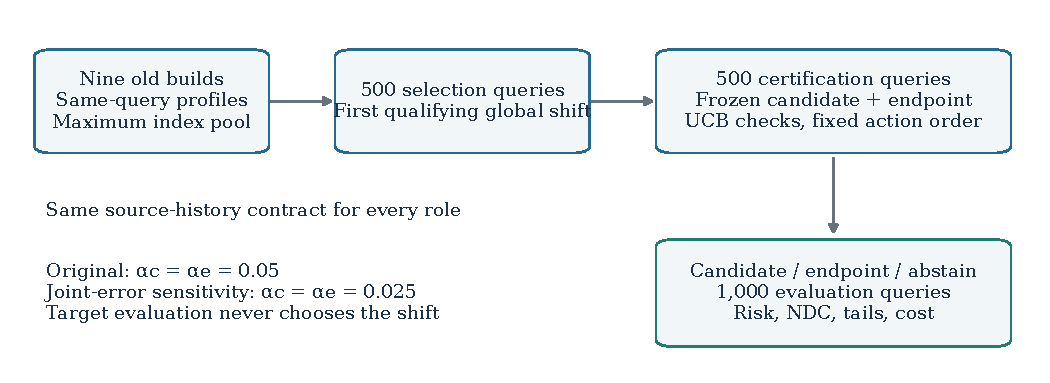
\includegraphics[width=\textwidth]{figures_v3/workflow.pdf}
\caption{ICBA applied to a recurring-query policy. Historical profiles construct candidates; target selection freezes one rule; certification chooses candidate, endpoint, or abstention; evaluation has no feedback path. The same interface also accepts fixed and target-global candidates.}
\label{fig:workflow}
\Description{Historical response profiles feed a candidate construction stage, followed by disjoint target selection, certification, and evaluation roles.}
\end{figure*}

\subsection{Source One-Rung as an Ablation}
\label{sec:slack-method}
A source-design role chooses the lowest native action whose Bonferroni-adjusted CP bound passes and then shifts it upward by one grid rung, clipping at the endpoint. Later source certification and target evaluation roles are disjoint. The rule uses no target selection, so it isolates whether source evidence leaves recoverable slack. A subsequent target-certified stage freezes that candidate before new certification and evaluation roles are accessed. The paired strong-baseline audit compares it with fixed-256 and target-global policies on the same prospective builds using new disjoint query roles. Its status is determined by that comparison, not by its absolute gain alone. On the registered 100K hnswlib grids the rule clips to the endpoint and saves no work, providing the bridge's no-slack counterexample.

\section{Experimental Design and Inference}
\label{sec:methodology}

\paragraph{Registered settings.}
SIFT-100K uses 128-dimensional Euclidean vectors; Arxiv-Nomic-100K uses 768-dimensional normalized inner-product vectors. The graph-only study uses 24 hnswlib and 24 Faiss builds per dataset, 750 queries, and all 552 non-diagonal directions. Native grids are $(10,20,40,80,120,200)$ for hnswlib and $(16,32,64,128,256,512)$ for Faiss. Deep1M uses eight hnswlib builds and grid $(200,300,400,600,800,1200)$. Native actions are never equated across implementations.

\paragraph{Evidence stages.}
The graph-only experiment executes each source first-passing action on the target and compares it with the target first-passing reference. A separate seed-991 refresh replaces 5\% of each 100K collection, rebuilds ten old and ten refreshed indexes, and replays one recurring-query policy. TCP uses 500 selection, 500 certification, and 1,000 evaluation queries.

After these analyses were frozen, the source one-rung boundary used previously untouched source-certification and target-evaluation roles. Post-seal Faiss and Deep1M studies added mutually exclusive target-certification and evaluation roles. The prospective confirmation then created eight new insertion-permutation builds per dataset and three 500-query roles, all frozen before response access. It retained the registered Faiss grid, fixed CPU, and source one-rung policy. The paired strong-baseline audit reused this prospective build panel but introduced another three disjoint 500-query roles. It is therefore a paired method comparison, not a second independent build campaign.

\begin{table*}[t]
\caption{Evidence provenance. ``Frozen before'' identifies when the candidate or analysis rule became immutable. Prospective confirmation and the paired audit share builds but use disjoint query roles.}
\label{tab:provenance}
\scriptsize
\begin{tabularx}{\textwidth}{@{}lcllX@{}}\toprule
Stage & Target builds & Query roles & Frozen before & Supported claim \\\midrule
Graph-only transfer & 24 per implementation/dataset & 750 shared & response analysis & response non-portability on fixed builds \\
Refresh replay & 10 matched old/new per dataset & 500/500/1,000 & target evaluation & policy deterioration and TCP recovery \\
Prospective confirmation & 8 new per dataset & 500/500/500 & build/query response access & per-target qualification and runtime value \\
Paired strong-baseline audit & same 8-build panel & new 500/500/500 & all arm responses & method attribution under matched builds \\
Deep1M replication & 8 registered & 500/500/500 & fresh-role access & target-certified scale evidence \\\bottomrule
\end{tabularx}
\end{table*}

\paragraph{Paired-audit arms.}
The deployable arms are endpoint-512; certified fixed-256; certified source one-rung; target-global with 250 selection plus 250 certification labels; and target-global with 500 plus 500 labels. Fixed-256 is the penultimate registered Faiss action, one rung below endpoint-512; it was predeclared as the largest non-endpoint fixed-action control before any paired-audit role or response was accessed. Diagnostic uncertified arms and an evaluation oracle attribute risk and headroom but cannot authorize deployment.

On the selection role, target-global retains actions whose one-sided CP UCB at Bonferroni level $0.05/6$ is at most $\delta=0.05$, then chooses the retained action with minimum mean NDC, breaking exact ties toward the smaller action. This screen constructs a candidate only. Deployment qualification comes from the disjoint certification role, where candidate and endpoint receive $\alpha_c=\alpha_e=0.025$; failed candidate certification executes the qualified endpoint, and endpoint failure causes abstention. The 500-label arm has the same target-label budget as source one-rung; source one-rung additionally uses its frozen historical profiles. The 1,000-label arm tests label value.

\paragraph{Metrics and timing.}
Risk is $\Pr(\rec@10<0.95)$. Serving gain is $1-\bar c_{\rm policy}/\bar c_{\rm endpoint}$ for NDC or wall-time, with equal query counts. We report pooled and per-target p95/p99, actual fallback, LOTO, and deletion sensitivities. Fixed-machine timing uses an AMD EPYC 7542, logical CPU 2 on NUMA node 0, Faiss 1.8.0 with AVX2, one search thread, 50 warmups per action, and seven interleaved repetitions measured by monotonic wall and process-CPU clocks. The primary cell value is the median of seven repetitions; crossed bootstraps resample target builds and query IDs while retaining repetitions within cells. Fallback timing executes the endpoint rather than splicing a counterfactual. Top-$k$ equivalence is required before timing contributes evidence; complete-cell fraction must be at least 0.99, median/max action-block CV at most 0.05/0.10, mean-gain interval lower bound above zero, p95-ratio upper bound at most 1.05, and every LOTO gain positive. An initial smoke showed that a per-query CV gate is not meaningful for sub-millisecond cells, where timer noise is large relative to the denominator. Before any candidate-versus-endpoint gain was inspected, only the measurement-validity rule was replaced by the action-block CV gate above; gain, tail, and LOTO thresholds were unchanged. The amendment, its failed-smoke record, and the resulting rule were hash-sealed before gain mapping and are reproduced in the supplement.

\paragraph{Inference.}
Primary recovery intervals use 5,000 seed-991 crossed bootstrap replicates over target builds and shared query IDs, retaining source directions within each target--query cell. Graph-only intervals resample query IDs with their complete directed-pair vectors. LOTO deletes one target without refitting. Seed 991 has separately recorded roles for query membership and bootstrap generation; the memberships and random streams are not reused as observations. Deep1M also uses 5,000 target-build bootstrap replicates with seed 991. External-method and Vamana intervals retain their native units. No pooled cross-protocol effect or common leaderboard is formed. Certificates control each fixed target decision; simultaneous coverage of a multi-target campaign would require a separately preregistered error allocation and is not claimed.

\paragraph{Questions.}
RQ1--RQ2 establish graph-only and refresh non-portability. RQ3 tests what ICBA authorizes. RQ4 spans endpoint-relative recovery, prospective confirmation, and the paired strong-baseline audit (Section~\ref{sec:recovery-results}). RQ5--RQ6 test tails and build sensitivity. RQ7 covers external methods, scale, and graph family. RQ8 separates measured runtime from modeled lifecycle cost. RQ9 audits reproducibility.

\section{Where Budget Portability Fails}
\label{sec:portability}

\subsection{RQ1: Do Responses Transfer When Only the Graph Changes?}
Retrospective first-passing actions frequently fail after a graph-only rebuild, even though collection membership, queries, and truth are unchanged. Table~\ref{tab:graph-only} reports absolute target risk, the unresolved-reference risk, and their difference. Across hnswlib and Faiss on both datasets, the increment ranges from 17.17 to 23.60 percentage points; every query-cluster interval is above zero. This is a response-level result independent of TCP's pooling or recalibration.

\begin{table*}[t]
\caption{Graph-only response transfer at $k=10$, $\tau=0.95$. Each row has 24 builds, 552 directed pairs, and 750 shared query IDs. Risk entries and increments are percentages or percentage points [95\% query-cluster interval], conditional on the fixed build set. The reference uses the target's own first-passing response; its failures are unresolved queries. Finite variation counts queries with at least two distinct finite first-passing actions, divided by all 750 queries.}
\label{tab:graph-only}
\small\begin{tabular*}{\textwidth}{@{\extracolsep{\fill}}llcccr@{}}\toprule
Implementation & Dataset & Absolute risk (\%) & Reference risk (\%) & Increment (pp) & Finite variation (\%)\\\midrule
\GraphOnlyRows
\bottomrule\end{tabular*}
\end{table*}

The variation is principally among finite budgets: 75.87--91.07\% of queries have different finite first-passing actions across builds, while only 0.53--2.67\% switch between resolved and unresolved states. Removing the 1\% of queries with largest incremental contribution leaves increments of 21.37 (hnswlib/SIFT), 16.95 (hnswlib/Arxiv), 23.43 (Faiss/SIFT), and 17.53 (Faiss/Arxiv) percentage points. Reference unresolved risk spans 0.07--8.82\% across the registered settings. The reported increment subtracts that reference risk, while deployment checks candidate and endpoint separately and abstains if the endpoint does not qualify. Endpoint censoring therefore cannot manufacture a qualified fallback; it instead narrows which registered grids support a decision. Together with the deletion result, this rules out censoring and a handful of extreme queries as explanations for the observed transfer loss.

This experiment diagnoses the budget--response relation using retrospective truth on both source and target. It establishes that source success alone is insufficient evidence for action reuse. The measured mechanism is behavioral variation across builds; structural attribution to particular edges or navigation paths lies outside this response-level design.

\subsection{RQ2: Does an Executable Policy Deteriorate after Refresh?}
The matched old/new replay holds the nine-history policy fixed and applies it to both snapshots. Unlike RQ1, this changes 5\% of the vectors as well as rebuilding. SIFT's empirical risk rises from 3.77\% to 6.69\%; Arxiv-Nomic's rises from 3.19\% to 7.24\%. The corresponding paired increments [crossed 95\% interval] are 2.92 [1.75, 4.07] and 4.05 [2.86, 5.31] percentage points. Thus this is a measured deterioration, not merely an absolute target risk with an unknown source baseline.

Independent single-policy CP checks at $\alpha=0.05$ qualify six of ten old SIFT policies and five of ten old Arxiv policies. All eleven fail the corresponding target check. This paired diagnostic uses per-policy checks rather than simultaneous control over the eleven transitions. Target evaluation risk exceeds 5\% in all ten builds of each dataset; removing the highest-risk target leaves 6.61\% and 7.13\%. The deterioration is distributed across targets.

The same policy information is held fixed in each old/new comparison, but the experiment does not separate changed graph paths from changed nearest-neighbor membership. Together, RQ1 and RQ2 establish complementary facts: unchanged data do not make the response function portable, and a recurring-query policy can lose its old qualification after refresh plus rebuilding.

\section{Audit Decisions, Recovery, and Strong Baselines}
\label{sec:recovery-results}

\subsection{RQ3: What Does ICBA Authorize?}
Direct unshifted reuse fails every candidate certificate in the original refresh replay and routes all 20 targets to the endpoint. ICBA therefore blocks uncertified efficiency without manufacturing a saving. TCP changes the candidate before certification. The original allocation accepts 19/20 candidates; the $0.025+0.025$ sensitivity accepts all ten SIFT and six Arxiv candidates, with four certified endpoint fallbacks and no abstention.

\begin{figure*}[t]
\centering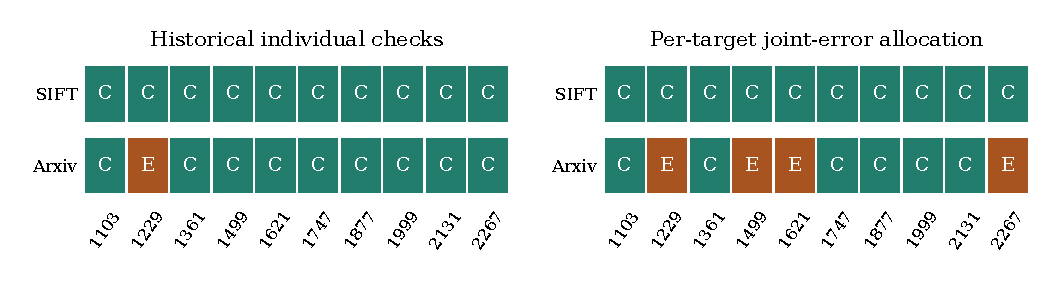
\includegraphics[width=\textwidth]{figures_v3/decisions.pdf}
\caption{Completed target decisions. C denotes candidate and E endpoint fallback. The left procedure uses historical individual $0.05/0.05$ checks and does not provide 95\% joint control for the completed choice. The right allocates $0.025/0.025$ per target, changing Arxiv composition from nine to six candidates.}
\label{fig:decisions}
\Description{SIFT accepts ten candidates under both rules. Arxiv accepts nine under the original allocation and six under the stricter allocation.}
\end{figure*}

\subsection{RQ4a: Endpoint-Relative Recovery and Incremental Value}
TCP's original completed decisions reduce mean NDC by 44.39\% on SIFT and 44.79\% on Arxiv. Under the joint-error allocation, SIFT is unchanged and Arxiv retains 29.86 [14.75,45.00]\%. Risk is 1.79\% and 1.68\%, respectively. Both remain positive relative to each target's endpoint.

The equal-target-label-budget comparison asks the stronger question. It is a post-hoc frozen-response sensitivity, not a preregistered confirmation. TCP and target-global each use 500 selection, 500 certification, and 1,000 evaluation queries; TCP additionally uses nine frozen historical per-query profiles. TCP gains a further 27.60 [17.92, 36.72]\% mean NDC on SIFT. Arxiv's gain is 10.78 [$-8.48$, 29.43]\%, while its p95 ratio is 1.109 [1.012, 1.285]. Historical query conditioning therefore adds resolved value only on SIFT under the registered event, grid, and SLA.

\begin{figure}[t]
\centering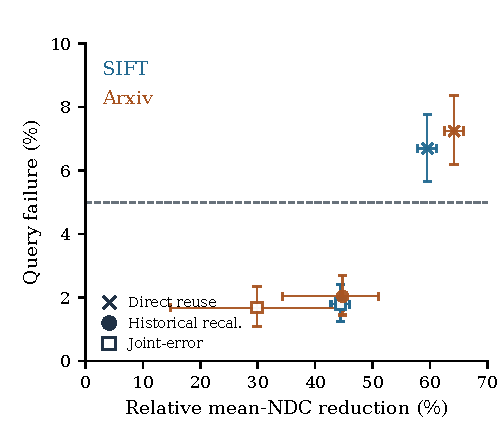
\includegraphics[width=\linewidth]{figures_v3/tradeoff.pdf}
\caption{Refresh risk--work tradeoff with crossed 95\% intervals. Marker shapes denote direct reuse ($\times$), historical recalibration ($\circ$), and the joint-error completed decision ($\square$); color denotes dataset. The endpoint is the zero-gain reference and is not plotted.}
\label{fig:tradeoff}
\Description{Direct reuse has high failure. Target-recalibrated policies have lower risk and retain positive search-work savings.}
\end{figure}

\subsection{RQ4b: Prospective Build Confirmation}
\label{sec:prospective}
\label{sec:fresh-bridge}
The prospective confirmation freezes source one-rung before eight new insertion-permutation builds and three new query roles per dataset are accessed. All 56 directed decisions per dataset accept the candidate, with zero fallback or abstention (Table~\ref{tab:s9-prospective}). Across 144,000 response cells and 112,000 raw timing measurements, native and measured top-$k$ agree exactly. Mean candidate/endpoint latency is 0.280/0.576 ms on SIFT and 1.161/1.662 ms on Arxiv. Sparse-grid and 2.5\%-risk sensitivities remain qualified but collapse to the endpoint, defining preregistered boundaries rather than failures of the primary configuration.

\begin{table*}[t]
\caption{Prospective confirmation on eight new target builds per dataset. C/F/A counts candidate/fallback/abstention. Risk and wall-time reduction are percentages [95\% crossed target-build/query interval]. p95 is the completed-decision/endpoint wall-time ratio [95\% interval]; LOTO is minimum wall-time reduction after deleting one target.}
\label{tab:s9-prospective}
\small\begin{tabular*}{\textwidth}{@{\extracolsep{\fill}}lrrrrr@{}}\toprule
Dataset & C/F/A & Eval. risk & Wall-time reduction & p95 ratio & LOTO reduction\\\midrule
\SProspectiveRows
\bottomrule\end{tabular*}
\end{table*}

Section~\ref{sec:paired-audit} next tests whether the confirmed source-specific complexity is necessary.

\subsection{RQ4c: Strong Baselines Change the Method Conclusion}
\label{sec:paired-audit}
The paired strong-baseline audit evaluates fixed and target-calibrated policies on the same prospective indexes with new disjoint roles (Table~\ref{tab:s9-baselines}). Every deployable arm passes the predeclared risk, mean wall-time, p95, LOTO, and timing-stability gates. Fixed-256 exactly matches source one-rung on SIFT. On Arxiv it provides 10.91 percentage points more wall-time reduction while both policies satisfy the declared 5\% risk contract. Source-specific tailoring is therefore unnecessary on this panel.

The equal-target-label-budget target-global-500 arm remains qualified and positive, but one of eight targets falls back, producing seven fallback cells among 56 directed comparisons and widening its interval. With 500 selection plus 500 certification labels, target-global-1000 achieves the largest measured wall-time reduction on both datasets. This is a label-value result, not evidence of superiority at a common total information budget. The nondeployable evaluation oracle leaves 21.81 mean-NDC gain points beyond target-global-1000 on SIFT; on Arxiv, the label-rich target arm reaches the oracle action pattern.

This paired audit compares frozen arms; it is not a deployment selector. Choosing an arm after inspecting these evaluation results requires a new certificate/evaluation cycle or a preregistered meta-selection rule.

\begin{table*}[t]
\caption{Paired strong-baseline audit. C/F/A counts candidate/fallback/abstention over 56 directed comparison cells (eight targets $\times$ seven source directions). For fixed and target-global arms, one decision and its labels are shared within each target; thus 49/7/0 denotes one target fallback repeated across seven cells, not seven independent target failures. Risk and wall-time reduction are percentages [95\% crossed target-build/query interval]; p95 is the completed-decision/endpoint wall-time ratio [95\% interval]; LOTO is minimum wall-time reduction. Target-global-500 uses 500 target labels; target-global-1000 uses 1,000.}
\label{tab:s9-baselines}
\scriptsize\begin{tabular*}{\textwidth}{@{\extracolsep{\fill}}lllrrrr@{}}\toprule
Dataset & Candidate & C/F/A & Eval. risk & Wall-time reduction & p95 ratio & LOTO\\\midrule
\SStrongBaselineRows
\bottomrule\end{tabular*}
\end{table*}

\paragraph{Mechanism attribution.}
Moving one rung above the source action lowers held-out risk from 2.15\% to 0.40\% on SIFT and from 1.775\% to 0.307\% on Arxiv, while sacrificing 24.92 and 31.21 percentage points of endpoint-relative mean-NDC reduction. These contrasts come from the paired diagnostic arms reported in the supplement. Certification changes authorization but not execution when every candidate passes. Target labels, rather than source-specific tailoring, drive the largest additional gains.

\subsection{RQ5--RQ6: Tail and Build Stability}
For historical joint-error TCP, pooled p95 is 2,349 versus 2,615 endpoint NDC on SIFT and 3,117 versus 3,252 on Arxiv; p99 is 2,774 versus 2,855 and 3,460 versus 3,504, respectively. Every target has non-increasing tails. The prospective confirmation and paired audit also pass p95 and LOTO gates; the least favorable paired-audit p95 upper bound is 0.930 for SIFT target-global-500 and 0.921 for its Arxiv counterpart. The conclusions therefore do not depend on one target build, although eight builds remain an underpowered basis for open-population inference.

\section{RQ7: Scope across Methods, Scale, and Graph Family}
\label{sec:families}

\paragraph{External adaptive methods.}
The frozen DARTH adapters produce target query-failure rates of 22.55\% on SIFT-100K and 23.12\% on Arxiv-Nomic-100K at $\rec@10<0.95$. Ada-ef yields 9.52 [9.44, 9.60]\% on ten Arxiv targets, with a target-build bootstrap conditional on its query set. All ten Ada-ef candidate certificates fail; audited execution uses the qualified endpoint and has zero search gain relative to that endpoint. Ada-ef is absent from Euclidean SIFT because the inspected estimator implements cosine/inner-product semantics, not a semantics-preserving L2 path. Its exclusion is an implementation-scope boundary, not a failed SIFT result.

These measurements show why query-risk qualification matters beyond TCP. Without matched source checks, they do not isolate rebuild-induced loss; their failure event also differs from mean recall and expected false-negative fraction. We therefore use them as qualification studies with their own information budgets.

\paragraph{Larger scale.}
On Deep1M, eight hnswlib builds cross four seeds with two insertion orders, giving 56 directed pairs on 1,000 queries. Source-derived first-passing actions have 28.86\% transport risk against 8.82\% target-reference risk. The incremental risk is 20.04 [17.29, 22.77] percentage points, using 5,000 seed-991 target-build bootstrap replicates conditional on the frozen source histories and query set. This is additional loss above a difficult, partly unresolved target reference.

A separate target-certified scale replication freezes three mutually exclusive 500-query roles and native actions 200, 300, 400, 600, 800, and 1,200 before access. All 56 source one-rung candidates separately qualify under per-target certificates. Held-out risk is 1.632 [0.804, 2.614]\%, endpoint-relative mean-NDC saving is 34.282 [33.533, 35.045]\%, and pooled p95/p99 ratios are 0.682/0.695. This extends target-certified recovery to one million vectors without converting it into a cross-implementation leaderboard.

\paragraph{Vamana-style evidence.}
Six source and six separate target builds produce 36 directions and 750 queries per dataset, using native search-list size and beam width one. The frozen event table combines its stage-specific under-budget and censoring outcomes. A target-build reanalysis gives 16.86 [15.88, 17.93]\% on SIFT and 11.37 [10.80, 11.99]\% on Arxiv. Its recorded responses do not reconstruct exactly the first-passing execution estimand used for hnswlib/Faiss. We retain it as directional cross-family evidence, not another row of Table~\ref{tab:graph-only}.

Vamana cost-tax intervals include zero: 1.07 [$-1.03$, 2.86]\% and 1.17 [$-0.83$, 3.03]\%, respectively, for the mean of per-target ratios in that reanalysis. Thus it supplies no established positive cost penalty or cross-engine superiority. Table~\ref{tab:scope} summarizes which question each setting can answer.

\begin{table*}[t]
\caption{Scope of the extension evidence. Each row retains its event, reference, and inference unit. All numeric intervals in the text are 95\%; no common cross-engine ranking or pooled effect is formed.}
\label{tab:scope}
\small\begin{tabularx}{\textwidth}{@{}lXXl@{}}\toprule
Setting & Event and reference & Supported comparison & Unit / query count\\\midrule
DARTH & Absolute target $\rec@10<0.95$ risk; no matched reference subtraction & Target qualification under the frozen adapter & Target summaries; 1,000/build\\
Ada-ef & Absolute target $\rec@10<0.95$ risk; endpoint for audited saving & Candidate rejection versus endpoint execution on Arxiv & 10 target builds; 1,000/build\\
Deep1M & Transport versus target reference; certified slack versus efSearch 1200 & Transfer loss and certified recovery at 1M scale & 8 targets; 1,000 prior + 1,500 fresh\\
Vamana-style & Frozen stage under-budget/censoring event; stage-specific cost reference & Directional cross-family transfer evidence, not a harmonized HNSW increment & 6 target builds; 750 shared queries\\\bottomrule
\end{tabularx}
\end{table*}

Together with RQ1, these results broaden the evidence without collapsing unlike estimands. Response non-portability appears across HNSW implementations and at larger scale; qualification changes the executable outcome of adaptive actions; and Vamana supplies directional graph-family evidence under a narrower event definition. The common conclusion is the need to bind a budget decision to its target index and risk contract.

\section{RQ8: Runtime and Lifecycle Value}
\label{sec:economics}

NDC is implementation-independent search work; elapsed time is the deployment endpoint. We therefore report both without substituting one for the other.

\paragraph{Measured fixed-machine runtime.}
The historical timing campaign covers the registered 24-build Faiss panel per dataset on the machine described in Section~\ref{sec:methodology}. The original sub-millisecond per-query CV criterion was rejected because timer noise dominated those cells. Before candidate-versus-endpoint gains were inspected, only measurement validity was amended to the action-block stability gate; gain, tail, and LOTO thresholds were unchanged and the amendment was hash-sealed before gain mapping. Source one-rung reduces wall-time by 9.44 [9.04, 9.77]\% on SIFT and 26.04 [25.62, 26.44]\% on Arxiv. p95 ratios are 0.988 and 0.914, and minimum LOTO reductions are 9.42\% and 25.97\%. These conservative 24-build estimates and the larger prospective-panel estimates use different build/query panels. The prospective confirmation and paired audit retain positive reductions on disjoint query roles evaluated over the same eight-build panel; they are not independent build replications.

\paragraph{Lifecycle accounting.}
For policy $\pi$ at horizon $N$,
\begin{equation}
 C_\pi(N)=C_{{\rm acquire},\pi}+N\bar c_\pi,
 \qquad N_{\rm BE}=\frac{\Delta C_{\rm acquire}}{\bar c_{\rm end}-\bar c_\pi}.
 \label{eq:breakeven}
\end{equation}
Cached history treats old profiles and truth as sunk; cold history charges their acquisition once per snapshot. Target selection, candidate and endpoint certification, and exact target truth are charged to recovery; truth is modeled as one scan of 100,000 vectors per labeled query. At $N=10^6$, cold-history joint-error TCP saves about 490 million NDC on SIFT and 389 million on Arxiv; break-even is approximately 396,000 and 457,000 executions, compared with 129,000 and 148,000 under cached history. Four Arxiv fallback targets do not individually amortize positive recovery overhead.

\begin{table}[t]
\caption{Joint-error TCP break-even executions in thousands [95\% target-build interval]. ``No saving'' counts nonamortizing targets.}
\label{tab:economics}
\small\begin{tabular*}{\linewidth}{@{\extracolsep{\fill}}llrr@{}}\toprule
Dataset & History & Break-even, $10^3$ & No saving\\\midrule
\CostRows
\bottomrule\end{tabular*}
\end{table}

The post-seal target-certified Faiss ledger charges one 500-query target audit per target and reuses it across 23 source histories. Pairwise accounting charges that audit to every directed source--target unit; shared-target accounting charges it once per target and reuses the distinct required actions across its 23 sources. Portfolio break-even [95\% target-bootstrap interval] is 66,914 [64,805, 69,940] and 17,018 [16,767, 17,276] executions under pairwise accounting, versus 3,019 [2,923, 3,157] and 755 [744, 767] under shared-target accounting for SIFT and Arxiv. Because 460/552 and 230/552 directions clip to the endpoint, pairwise ratios are portfolio thresholds, not per-direction guarantees; the worked ledger is in the supplement.

Target-global-500 uses 500 target labels, equivalent to 50 million exact-distance computations per target under the same truth model; target-global-1000 doubles both labels and truth work. Their end-to-end wall-time break-even is not claimed because truth and control wall-time were not recorded. Historical source acquisition and exact-truth/control wall-time are likewise unavailable and are not assigned zero. Measured timing establishes serving-latency reduction on one machine; it does not convert either NDC ledger into a hardware-general monetary claim.

\begin{figure}[t]
\centering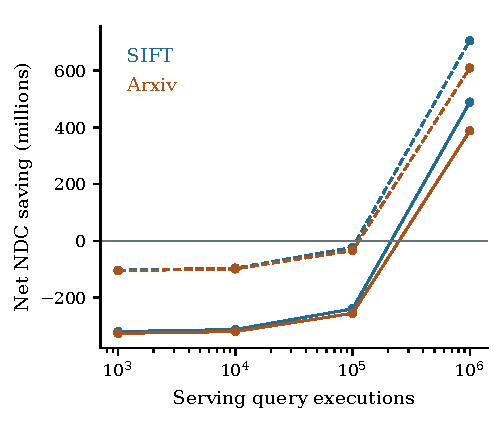
\includegraphics[width=\linewidth]{figures_v3/cost.pdf}
\caption{Modeled joint-error TCP net distance saving versus serving horizon. Cold history crosses zero later than cached history; fallback targets remain in the average.}
\label{fig:cost}
\Description{Net distance savings become positive only after the acquisition cost is amortized over a sufficiently long serving horizon.}
\end{figure}

\section{Reproducibility, Scope, and Operational Rule}
\label{sec:discussion}

\subsection{RQ9: Can the Decision Chain Be Replayed?}
The anonymous artifact is self-contained and uses only declared dependencies. A clean environment imports no main-repository code, rebuilds the paper and supplement, and regenerates five main-paper figures and five data-linked tables. A fresh Faiss environment reproduces registered native action rows with zero top-$k$, recall, NDC, or action-order mismatch. The two prospective stages add 288,000 response cells and 112,000 raw timing measurements with zero top-$k$ mismatch. Role manifests verify zero overlap among selection, certification, and evaluation.

All records are committed with checksums and deterministic regeneration scripts; numeric claims are bound to repository records rather than generated prose. The anonymous artifact URL is supplied through the submission system.

\subsection{What the Evidence Establishes}
Across the registered builds, grids, query populations, and SLAs, budget response changes under graph rebuilds and data refresh, with scoped extensions across implementations and scale. ICBA detects this change and converts a frozen candidate into a target-qualified completed decision. TCP recovers endpoint-relative work for recurring profiled queries and adds resolved value beyond target-global calibration on SIFT under the same target-label budget, while using nine historical profiles. Target-global calibration is the stronger default on Arxiv. Source one-rung can work, but the paired audit shows that a fixed action can match it or provide greater efficiency while both policies satisfy the risk contract.

The resulting maintenance rule has three steps. First, audit inherited policies against the target event and endpoint. Second, certify the least complex viable candidate and its fallback on disjoint target queries. Third, escalate from fixed to target-global to query-conditional policies only when held-out gain and lifecycle accounting justify the additional information.

\subsection{Boundaries}
The main conclusions are conditional on registered query populations, grids, SLAs, and build panels. The prospective panel has eight builds per dataset and one CPU configuration; the paired audit reuses that build panel for attribution. TCP assumes recurring profiled queries. The complete cold-history ledger is expressed in NDC, while actual timing covers serving search rather than truth acquisition, control, energy, or storage. DARTH, Ada-ef, Deep1M, and Vamana retain different native estimands and support scope rather than a common ranking. These boundaries define the next replication targets without changing the fixed-target decisions reported here.

\section{Conclusion}
For the registered builds, grids, and query populations, search-budget portability is an index-conditioned deployment decision. ICBA makes that decision auditable by separating candidate construction, target certification, fallback, held-out evaluation, and cost. The evidence rejects automatic reuse, confirms qualified recovery on new registered builds and query roles, and shows why strong simple baselines are essential: fixed-256 can match or outperform source one-rung under the common contract, target calibration provides the largest measured gains on the paired panel, and TCP is valuable when recurring query histories add measurable information. The fixed-machine wall-time results apply to the recorded CPU and thread setting. The practical outcome is a complexity-aware policy ladder backed by target evidence rather than a universal recovery rule.

\balance
\bibliographystyle{ACM-Reference-Format}
\bibliography{references_final_v3}
\end{document}
